\documentclass[12pt,a4paper]{article}

\usepackage{inputenc}
\usepackage{textcomp}
\usepackage{amsmath, amssymb, amsfonts}
\usepackage[parfill]{parskip}
\usepackage{graphicx, subfig}
\usepackage{listings}
\lstset{language=Python, breaklines=true}   

%\usepackage{natbib}
\usepackage[style=numeric,natbib=true,sortcites=true,block=space]{biblatex}
\bibliography{bibliography}

\title{A Step-Integrate Program for the CRIMI}
%\subtitle{, the Vacuum Fourier Transform Spectrometer}
\author{Ellen Schallig}

\begin{document}
 
\maketitle

 \begin{abstract}
 For the `FIT-stage' (small internship) I have made software for a Fourier transform spectrometer. This is a stand-alone program which works with the step-integrate method: each step of the stage is followed by dwell time and a measurement, after which another step is taken. Some work has been done involving the fast scan method, however, most of this remains future work.
 \end{abstract}

%%%%%%%%% NEW SECTION: INTRODUCTION %%%%%%%%%

\section{Introduction}
The CRIMI (ChRIs $\&$ MIchelson) is an infrared Fourier transform spectrometer, made by Chris de Jonge, under supervision of Dr. Andrey Baryshev. The spectrometer is designed to be used in a vacuum, as water molecules and other abundant molecules absorb large parts of the infrared spectrum.

The goal of this internship was to write software to guide the linear stage in the CRIMI in making measurements, design a graphical user interface for easy user access and do some data processing on the acquired data: fast Fourier transforms and windowing. As a result, I have written a program in Python that automatically takes a complete measurement with this spectrometer. The program has scan length and stepsize, or equivalent resolution and maximum frequency, for input, and outputs the raw data in \verb!csv! format.

%Doe hier ook een plaatje van een FTS (kun je van WIKIPEDIA halen). doel van je stage was:
%aansturing van linear stage
%grafische user interface
%data processing (FFT algorithmes + windowing)
%Zet in deze introductie ook een formule en plaatje met spectrum en interferogram.
%\textbf{Verder is het goed om hier ook aan te geven hoe padlengte de resolutie bepaalt, en minimale stapgrootte de hoogste frequentie.}

\subsection{Fourier Transform}

Fourier transform spectrometers (FTS) work on the interference and Fourier principles. The spectrometer has a moveable part and stationary parts. In the case of figure~\ref{fig:fts}, a moving mirror provides a difference in distance travelled by the two beams of light created by the beamsplitter. By moving one mirror, the path length $l_1$ is made different from $l_2$, which produces an interference pattern when the light is recombined. This pattern is a cosine wave for each wavelength. Because of the range of wavelengths in the source, at different positions of the mirror, different wavelengths are attenuated.

\begin{figure}
 \begin{center}
  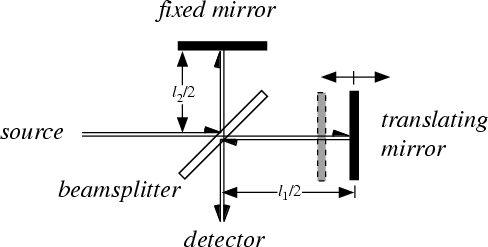
\includegraphics[width=0.8\textwidth]{figures/fts.png}
  \caption{A simple Fourier transform spectrometer (FTS). Path length differences are created by moving parts of the setup.  From \cite{wolf}.}
  \label{fig:fts}
 \end{center}
\end{figure}


With a Fourier transform the intensity for each position ($\delta$) is turned into the intensity for each wavenumber ($\tilde{\nu}$), because one is the inverse of the other: $\tilde{\nu} = \frac{1}{\delta}$, and from this the frequency $f$ can be computed: $\tilde{\nu}\cdot c=f$. $\delta$ and $\nu$ are together called a Fourier transform pair.

The Fourier transform of a function is the following formula:

\[
 F(\omega)=\int_{-\infty}^{\infty}f(t)e^{-i\omega t}dt,
\]
with $i$ the unit imaginary number. However because all wavelengths produce cosine waves, the total input is just a summation of cosines. Also we talk about position and wavenumber, so in this case the Fourier transform can be simplified to

\[
 F(\tilde{\nu}) = \int_{-\infty}^{\infty}f(\delta)\cos(2\pi\delta\tilde{\nu})d\delta,
\]

with $F(\tilde{\nu})$ the power of the source as a function of wavenumber or frequency, and $f(\delta)$ the power as a function of path length difference.

Because of this Fourier transform and $\tilde{\nu} = \frac{1}{\delta}$, a longer path length for the measurement causes a higher resolution, and a smaller stepsize gives a higher highest frequency.

\begin{figure}
 \begin{center}
  \subfloat[The measured interferogram.]{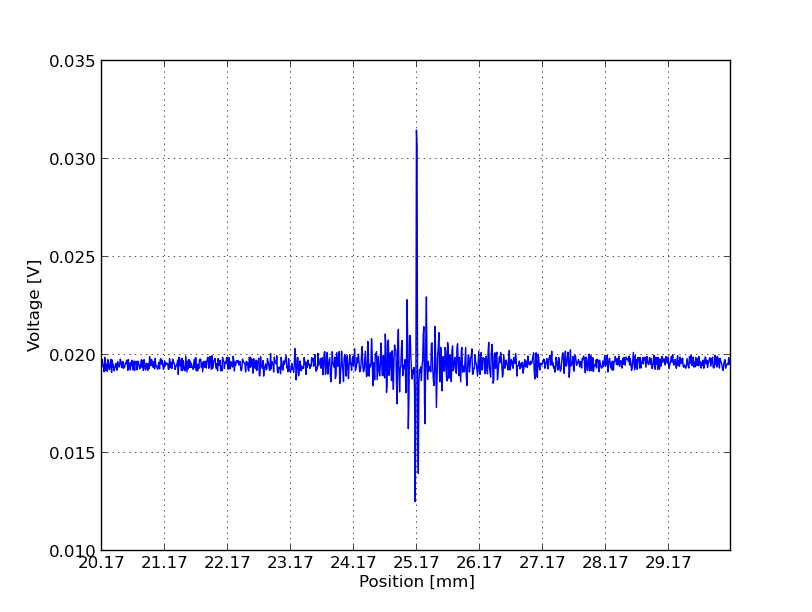
\includegraphics[width = 0.47\textwidth]{figures/interferogramforreport.png}}
  \quad
  \subfloat[The spectrum.]{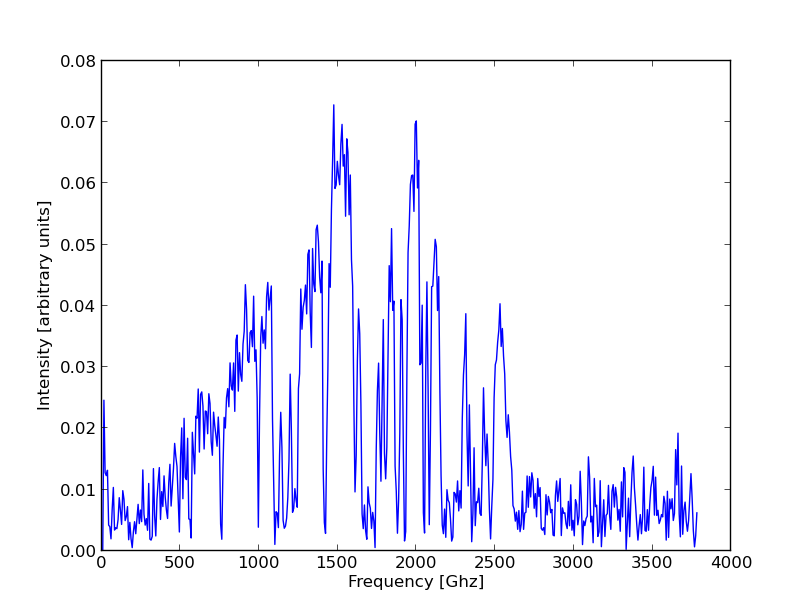
\includegraphics[width = 0.47\textwidth]{figures/fourierplotforreport.png}}
  \caption{The Fourier transform of an interferogram gives the spectrum.}
  \label{fig:fouriertransform}
 \end{center}
\end{figure}

\subsection{Hardware}

The spectrometer needs a few devices to function (see figure \ref{fig:hardware}). The controller to move the stage in is the PI C867.160 controller. The lock in amplifier in use is the SR510. A third device is needed to be able to communicate with the lock in amplifier from any computer: a GPIB-Ethernet adapter. This device counteracts the need for a special GPIB circuit card in the computer. All three are hardcoded into the software. This means unfortunately that the software does not automatically work with e.g. the SR530 lock in amplifier, or with a direct GPIB connection to the computer.

The test setup used a helium-cooled bolometer to actually measure the power of the radiation. This report will not deal any further with the measuring device, as the software is independent of that.


\begin{figure}[h!tb]
	\begin{center}
		\subfloat[The controller for the stage from PI.]{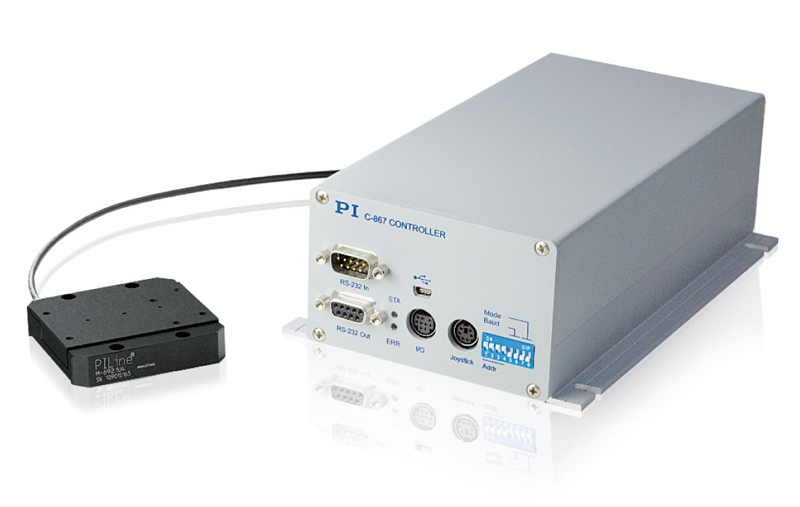
\includegraphics[width = 0.45\textwidth]{figures/pi_c867_160.jpg}}
		\qquad
		\subfloat[The SR510 lock in amplifier.]{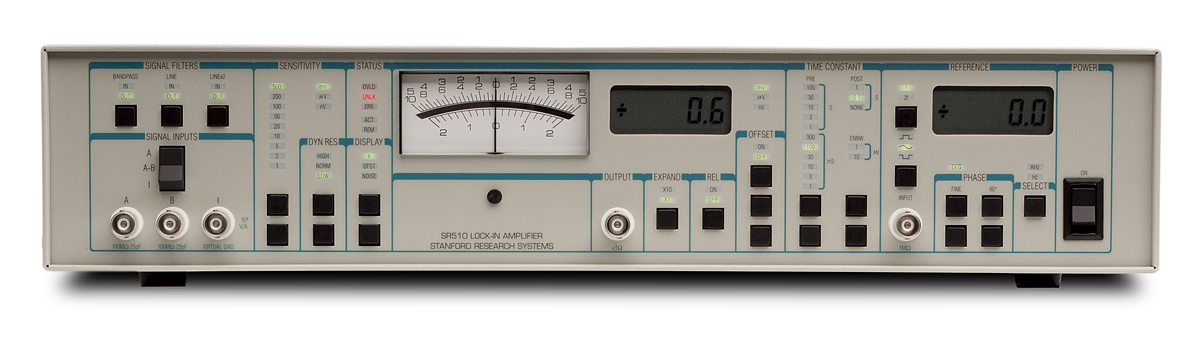
\includegraphics[width = 0.45\textwidth]{figures/SR510_FPlg.jpg}}
		\qquad
		\subfloat[The GPIB-Ethernet Controller.]{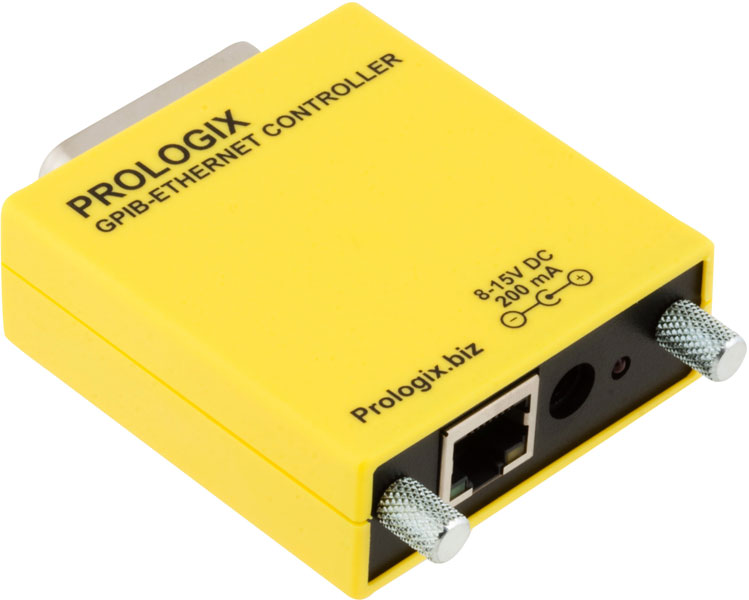
\includegraphics[width = 0.4\textwidth]{figures/GPIB-Ethernet-back.jpg}}
		\caption{The hardware. Pictures from \cite{PI}, \cite{SR}, and \cite{prologix}.}
		\label{fig:hardware}
	\end{center}
\end{figure}

It is important to mention that on the SR510 the DIP-switches need to be in a different configuration than the `example' configuration as mentioned in its manual on page 7. For fast readout, SW1 switch 6 should be in the `up' position instead of in the `down' position, to suppress echoing over the RS232 connection (which is unconnected in this setup). The SW2 switches are not of importance in this setup, as no RS232 connection is used. See figure~\ref{fig:SR510_back} for the location of this switch.

\begin{figure}[h!tb]
 \begin{center}
  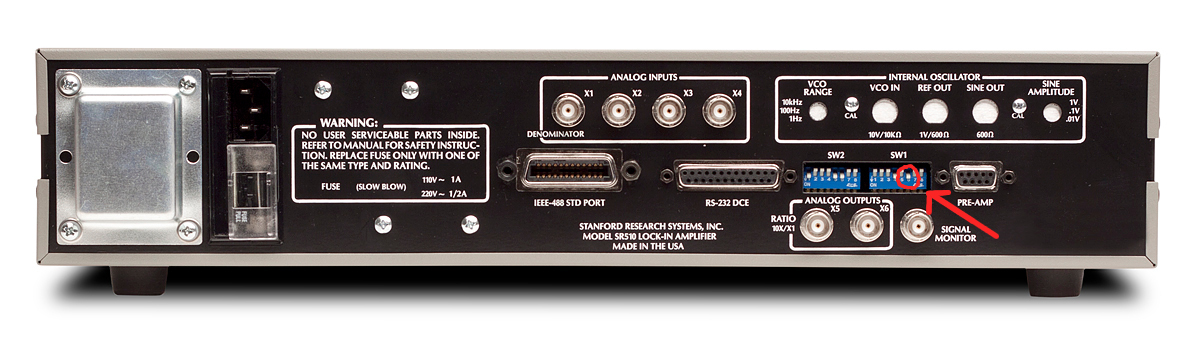
\includegraphics[width=\textwidth]{figures/SR510_Rear_circle.jpg}
  \caption{The back plate of the SR510 lock in amplifier. Encircled is SW1 switch 6. For fast performance, this switch should be in the `up' position. Picture from \cite{SR}.}
  \label{fig:SR510_back}
 \end{center}
\end{figure}


The software is written for Windows, because almost all the computers at SRON make use of Windows. This is hardcoded, because only the COM-ports (serial ports) are coded in.

\subsection{Python}
Python is an interpreted, interactive, object-oriented programming language \cite{python}. It is open source and free, and easy to learn. Python runs on Windows, Linux/Unix and Mac OS X. It has an active community that contributes a large number of libraries for various tasks, e.g. numerical mathematics and hardware interfacing.

Python has the distinct advantage over programming languages such as LabVIEW that it is backwards compatible. Old code written in previous versions is in many cases still executable in newer Python versions, and as the files are plain text, it will be always readable in any editor. So even when old code cannot be executed anymore, it can still be modified to comply with newer standards.

This software is written in Python version 2.7. The extra (non-native) packages needed for the program are \verb!PySerial! to open a serial port for the PI-controller and \verb!wxPython! to make the GUI. For this last task \verb!wxFormbuilder!, an open source GUI designer which emits Python code, was also used. The other imported packages are part of the core Python distribution.

%%%%%%%%% NEW SECTION: STEP-INTEGRATE PROGRAM %%%%%%%%%

\section{Step-Integrate Program}

%Geef hier een blokdiagram van je programma, waarin aangegeven wordt hoe de data wordt ingevoerd, hoe de scan wordt uitgevoerd en hoe de data storage en processing (FFT, WIndowing, complex FFT?) wordt gedaan. Ter verduidelijking van de processing zou je een dummy interferogram (b.v. een top-hat) door je data processing kunnen sturen , om aan te geven wat het effect van de windowing is (en evt. het effect als je niet een correcte zero path hebt)

The code consists of a few different classes that talk to the hardware, or do measurements with the returned parameters. The classes \verb!C876_160!, \verb!SR510!, and \verb!EthernetAdapter! do the interaction with the hardware, with the commands as dictated in the corresponding manuals. The classes \verb!Parameters!, \verb!Plotting!, and \verb!Fourier! interact with the data that comes from the instruments. \verb!ReadoutSession! does the actual measurements, and a \verb!NepSession! has been made to test the rest of the code without having to use the actual hardware. The code comes together in the class \verb!Frame1!, where the different actions are coupled to the buttons in the GUI. This class also makes use of the file \verb!gui_stepintegrate.py!, which is the code for the GUI as generated by wxFormbuilder. See also figure~\ref{fig:blokdiagram}.


\begin{figure}[h!tb]
 \begin{center}
  \includegraphics[width=\textwidth]{figures/blokdiagram_classes.pdf}
  \caption{The classes in use in the program. The class `NepSession' is for testing purposes only.}
  \label{fig:blokdiagram}
 \end{center}
\end{figure}

\subsection{Addresses}
A few addresses have been hardcoded into the software. The stage controller is hardcoded to be on the (virtual) COM 3 port. The EthernetAdapter should have host '192.168.11.201' and port 1234, with the ethernet card in the computer the address '192.168.11.200'. Finally the lock in amplifier has to have GPIB address 8, because the EthernetAdapter is coded that way.


%%%%%%%%% NEW SECTION: GRAPHICAL USER INTERFACE %%%%%%%%%

\section{Graphical User Interface}
\begin{itemize}
 \item grafische user interface! wx, wx-python, wat gebeurt er in de code van de interface en hoeveel is het door elkaar gegaan met het programma zelf? wat zit er in de interface verwerkt, wat kan het programma doen?
\end{itemize}

\subsection{Walkthrough}

To start the program, click the icon or in the command window go to the correct folder and type \verb!python program_stepintegrate.py!. A window pops up with four frames, a `Welcome' frame, one to set the correct switches on the SR510 lock in amplifier, one for the measurement input and a frame to start the actual measurement.

\subsubsection{Welcome}

\begin{figure}[!ht]
 \begin{center}
  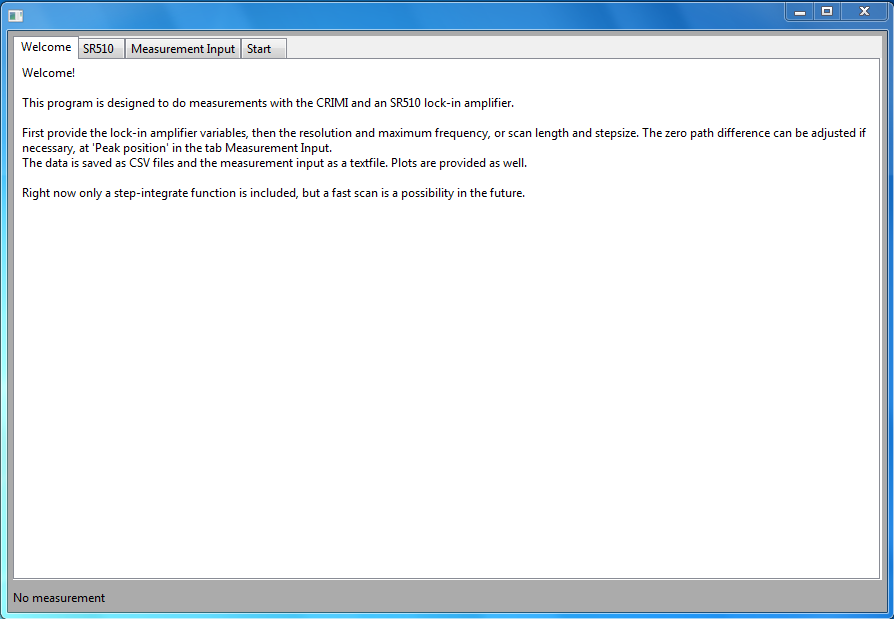
\includegraphics[width=0.8\textwidth]{figures/gui1}
  \caption{The GUI, frame 1: Welcome.}
  \label{fig:gui1}
 \end{center}
\end{figure}

Figure \ref{fig:gui1} shows the welcome screen with a short explanation on how to use this program. For the longer explanation, please read on.

\subsubsection{Setting the SR510 Lock In Amplifier}

\begin{figure}[!ht]
 \begin{center}
  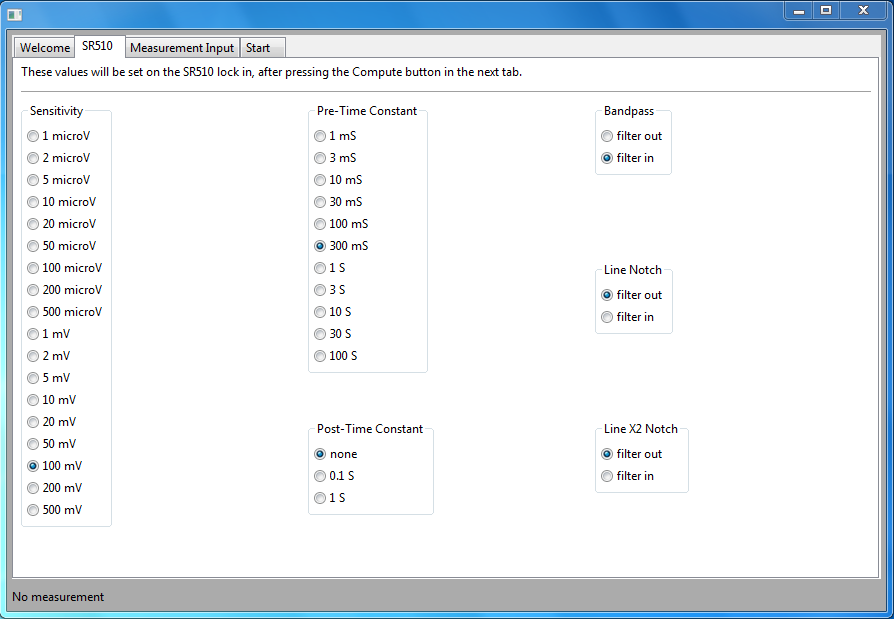
\includegraphics[width=0.8\textwidth]{figures/gui2}
  \caption{The GUI, frame 2: Setting the SR510 lock in amplifier.}
  \label{fig:gui2}
 \end{center}
\end{figure}

The second frame of the program, as shown in figure \ref{fig:gui2}, gives the most important features of the SR510 to set for the measurement. These settings are saved in a text file when the measurement is saved (see section \ref{subsub:saving} for more on saving the measurement data). Other settings can be changed on the lock in amplifier directly, but these settings will not be saved in the text file. The commands will be sent to the device after the button `Compute values and set SR510' in frame 3 has been pressed. The settings shown are the default values.

\subsubsection{Setting the Parameters for the Measurement}

\begin{figure}[!ht]
 \begin{center}
  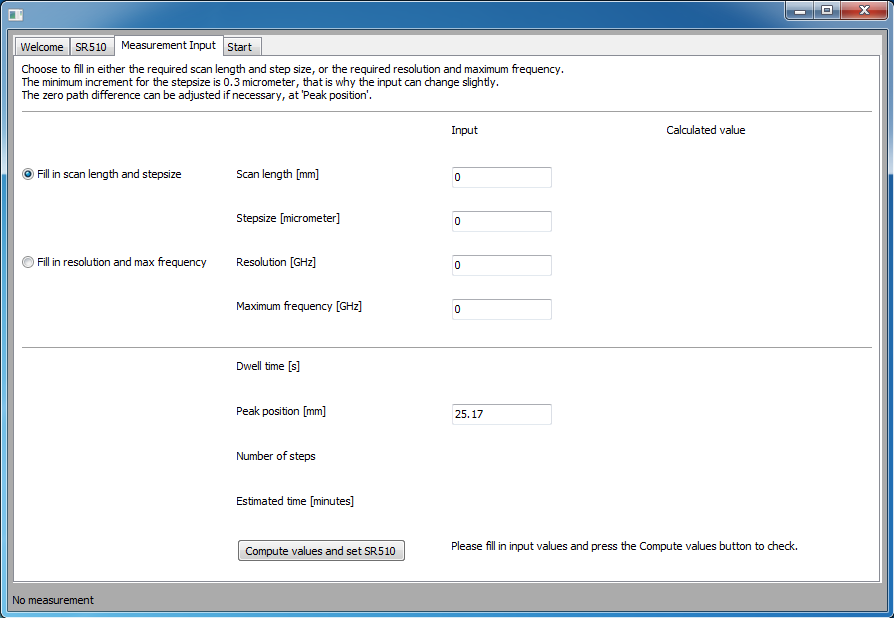
\includegraphics[width=0.8\textwidth]{figures/gui3}
  \caption{The GUI, frame 3: Setting the desired measurement input.}
  \label{fig:gui3}
 \end{center}
\end{figure}

In this frame (see figure \ref{fig:gui3}) the measurement input can be set. One can choose to fill in either the scan length and stepsize or the resolution and maximum frequency. The program converts this after pressing the `Compute values' button.

The discrepancies in the entered values and the computed values are because of the minimum stepsize of 0.3 micrometer that the stage can make. The code is designed such that the rounded values always represent a higher accuracy in the measurements than the provided values (e.g. smaller stepsize or higher resolution).

The zero bias point is experimentally found to be at a distance of 25.17 cm from the beginning of the stage. It can be adjusted easily by changing the value for the `Peak position'. Figure~\ref{fig:peakposition} shows a scan around the center, taken at a later moment. This plot shows that the value of 25.17 is not far off. A higher precision can be attained by tuning this zero bias point.

\begin{figure}[!ht]
 \begin{center}
  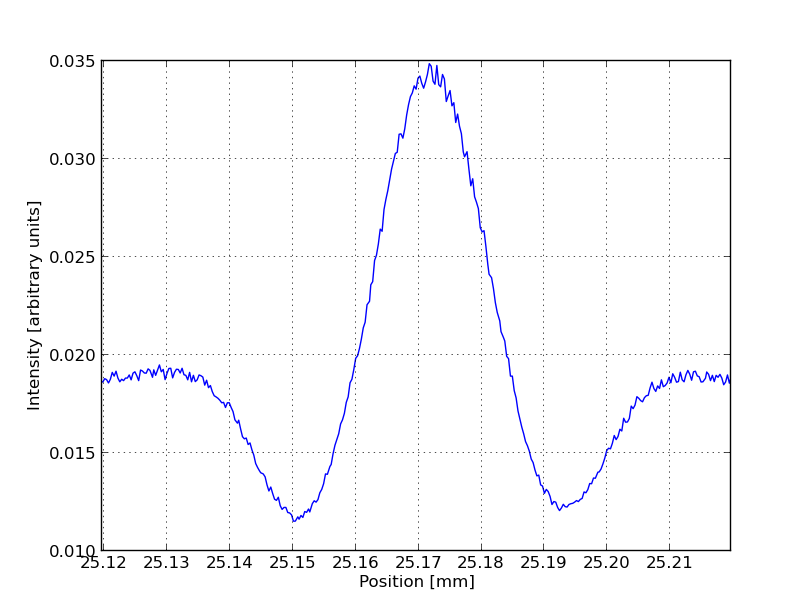
\includegraphics[width=\textwidth]{figures/peakposition}
  \caption{Experimental determination of the zero bias position.}
  \label{fig:peakposition}
 \end{center}
\end{figure}


\subsubsection{Starting and Saving the Measurement}\label{subsub:saving}

\begin{figure}[!ht]
 \begin{center}
  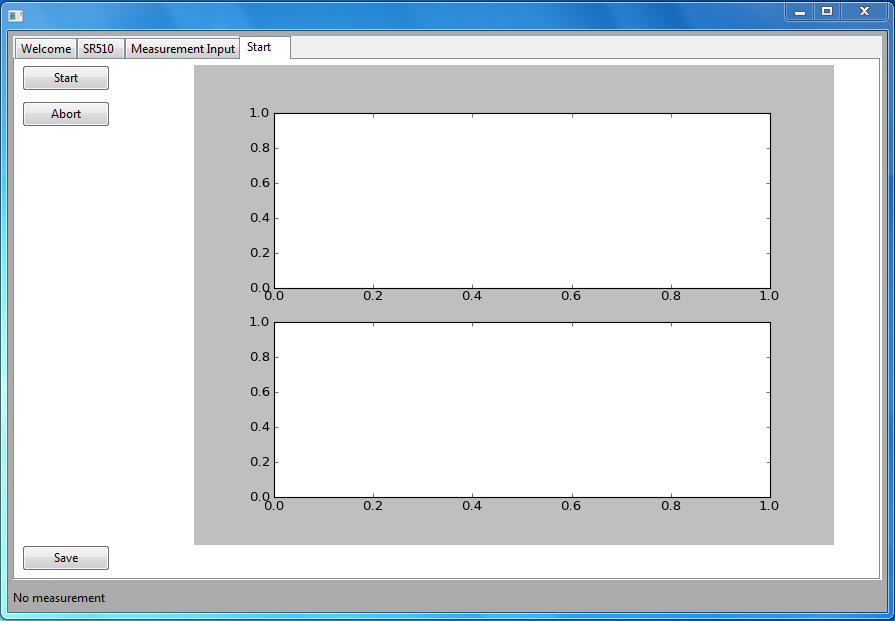
\includegraphics[width=0.8\textwidth]{figures/gui4}
  \caption{The GUI, frame 4: Starting the measurement, a plot of the measured points, and saving the data afterwards.}
  \label{fig:gui4}
 \end{center}
\end{figure}

\subsubsection{Examples}
\begin{itemize}
 \item Hier voorbeelden van wat er uit zo'n measurement komt, wat je kunt opslaan.
\end{itemize}

%%%%%%%%% Further Work %%%%%%%%%

\section{Possible Improvements}

I have created a working program for the CRIMI that takes measurements with the step-integrate method. This introduces waiting time, which can add up to hours for a precise measurement. To facilitate these kinds of measurements, a fast scan method could be implemented.

\subsection{Fast Scan}
Ideally with the fast scan method the linear stage moves between two specified end points and sends out a trigger pulse when a measurement should be made. At that moment it knows its position and this is sent to the computer, along with the voltage reading from the read-out device. In this way the same amount of data points can be acquired in much less time than is needed for the step integrate method. Even though this data is less precise, with these many more data points it does not matter much.

I started working on this, but have not yet managed to synchronize the stage and the read-out device, which is essential to make this method work. In this setup the read-out device was the Agilent 34401A multimeter. The controller for the stage can send these trigger pulses, but the multimeter side does not yet react to these pulses.

\subsection{Improvements to Code}
Even though the step-integrate program works, this does not mean that the code is perfect. In the class for the GUI (\verb!Frame1!) a few too many lines which should be in a new class slipped in. Especially where the different data files are saved, the GUI code and processing code are too much mingled. This saving process should be completely separated from the GUI.

In the same way in the GUI code the plotting during the measurement is done with different code than the plotting that is done during saving. This could be cleaned up by refactoring this part of the code.

In the \verb!Parameters! class some parameters are converted into different parameters. I tested the correctness by hand for the edge cases I could think of, but it would be better to write a unit test that can do this every time a small change is made in the code. 


%\begin{itemize}
%\item inhoudelijk: fast scan. wat heb ik tot nu toe gedaan, en waar wil ik heen. Was toch wel lastig.
%\item in de code: in het gui-gedeelte: het plotten uitdrukken in de plotmethodes die ik gemaakt heb, ipv dat stukje code `opnieuw' uit te werken.
%\item in de code: tests toevoegen om alle mogelijke manieren van afronden (bijv) te kunnen controleren en dus zeker weten dat dat stukje code doet wat je wilt dat het doet.
%\item nog meer de GUI loskoppelen van het data verwerken, vooral in het opslaangedeelte. Dat had een aparte klasse moeten worden.
%\end{itemize}

%14:03 <marten> of alleen al iets wat dan specifiek "acceptatietest" heet: sluit 
%               alles aan, op een bepaalde (simpelste) configuratie (bijv niet 
%               vacuum), en draai script die je vertelt of het apparaat lijkt te 
%               reageren zoals je dan zou verwachten (binnen bepaalde marges)
%14:04 <marten> dus iets wat niet randgevallen checkt, maar juist kijkt of alles 
%               in het simpelste geval nog werkt
%14:04 <marten> dat kun je dan ook gebruiken om te kijken of er geen motoren 
%               stuk zijn gegaan na een jaar op de plank
%14:04 <marten> en of je alles correct hebt aangesloten
%14:05 <marten> met het idee dat als die test slaagt, dat je dan m kunt gaan 
%               gebruiken voor je specifiek gewenste setup
%14:05 <marten> en met redelijke zekerheid kunt zeggen dat je logische 
%               resultaten zult krijgen



%%%%%%%%%% NEW SECTION: CODE DESCRIPTION %%%%%%%%%

\section{Code Description}
Leg key stukjes van de code uit, voor non-pythonners. Is dit nodig? Dat weet ik niet :(

%\appendix
%\section{Source Code}
%code!


\printbibliography

\end{document}